\documentclass[aspectratio=169]{beamer}
% Alternatives (use the one that matches your projector/screen best):
% \documentclass[aspectratio=43]{beamer}   % 4:3
% \documentclass[aspectratio=11]{beamer}   % 1:1 (will waste space on 16:9 screens)

% ===================== Theme =====================
\usetheme{Madrid}
\usecolortheme{default}
\usefonttheme{professionalfonts}
\setbeamertemplate{navigation symbols}{}
% Remove the default footline to gain vertical space (poster-style)
\setbeamertemplate{footline}{}

% ===================== Packages =====================
\usepackage{amsmath,amssymb,amsfonts}
\usepackage{booktabs}
\usepackage{graphicx}
\usepackage{url}
\usepackage[most]{tcolorbox}
\usepackage{anyfontsize} % allow explicit tiny font sizes

\newcommand{\TitleSize}{\fontsize{18}{24}\selectfont}
\newcommand{\FrameTitleSize}{\fontsize{12}{14}\selectfont}
\newcommand{\MainSize}{\fontsize{8}{7}\selectfont}
\newcommand{\CardTitleSize}{\fontsize{10}{12}\selectfont}
\newcommand{\TinyCap}{\fontsize{8.0}{9}\selectfont}

\setbeamerfont{title}{size=\TitleSize,series=\bfseries}
\setbeamerfont{frametitle}{size=\FrameTitleSize,series=\bfseries}
\setbeamerfont{normal text}{size=\MainSize}
\setbeamerfont{block title}{series=\bfseries}

% ===================== Compact layout =====================
\setlength{\abovedisplayskip}{1.5pt}
\setlength{\belowdisplayskip}{1.5pt}
\setlength{\abovedisplayshortskip}{1pt}
\setlength{\belowdisplayshortskip}{1pt}
\setlength{\parskip}{0pt}
\setlength{\columnsep}{1.15cm}  % more gutter between columns

% Leave width slack so columns don't "stick" visually
\newcommand{\colw}{0.475\textwidth}

% --- Make columns fill the available frame height and distribute spacing evenly
\newcommand{\ColH}{0.83\textheight} % tune: 0.80–0.86 works well depending on frametitle height

\newenvironment{colfill}[1]{%
  \begin{minipage}[t][\ColH]{#1}\raggedright
}{%
  \end{minipage}
}
% Optional: shorter alias
\newcommand{\spacer}{\vfill}


% ===================== Card style =====================
\definecolor{CardBG}{RGB}{250,250,252}
\definecolor{CardFrame}{RGB}{40,40,60}
\definecolor{CardAccent}{RGB}{30,90,160}
\definecolor{CardWarn}{RGB}{160,60,30}
\definecolor{CardGood}{RGB}{20,120,80}

\tcbset{
  enhanced,
  colback=CardBG,
  colframe=CardFrame,
  boxrule=0.45pt,
  arc=2mm,
  before skip=0.45mm, after skip=0.45mm,
  left=1.0mm,right=1.0mm,top=0.75mm,bottom=0.75mm,
  fontupper=\MainSize,
  fonttitle=\bfseries\CardTitleSize,
}

\newtcolorbox{card}[2][]{title={#2},colframe=CardFrame,#1}
\newtcolorbox{cardA}[2][]{title={#2},colframe=CardAccent,#1}
\newtcolorbox{cardW}[2][]{title={#2},colframe=CardWarn,#1}
\newtcolorbox{cardG}[2][]{title={#2},colframe=CardGood,#1}

% ===================== Figure helpers =====================
\newcommand{\FIGDIR}{/figures/}
\newcommand{\tryfig}[1]{\FIGDIR#1}
\newcommand{\safefig}[2]{%
  \IfFileExists{\tryfig{#1}}{%
    \includegraphics[width=\linewidth,height=0.34\textheight,keepaspectratio]{\tryfig{#1}}%
  }{%
    \IfFileExists{figures/#1}{%
      \includegraphics[width=\linewidth,height=0.34\textheight,keepaspectratio]{figures/#1}%
    }{
    }
  }%
  \vspace{-0.25em}\par{\TinyCap #2}%
}

% ===================== Meta =====================
\title[GFlowNet-BO]{GFlowNet-Guided Dropout Mask Sampling for Neural Bayesian Optimization}
\author{Anuar Aimoldin}
\institute{Course Project Presentation\[-0.2em]\TinyCap Learned dropout-mask generation for neural Bayesian optimization under a controlled evaluation protocol}
\date{}


\begin{document}

% ------------------------------------------------
\begin{frame}
  \titlepage
  \vspace{-0.7em}
  \begin{center}
    {\TinyCap Central claim: learning a distribution over dropout masks can help neural BO in some settings, but under a controlled protocol the benefit is benchmark-dependent rather than universal.}
  \end{center}
\end{frame}

% ------------------------------------------------
\begin{frame}{Problem, gap, and project question}
\vspace{-0.55em}
\begin{columns}[T,onlytextwidth]
\column{0.47\textwidth}
\begin{minipage}[t][0.82\textheight]{\linewidth}\vspace{0pt}
  \begin{cardA}{Why this problem matters}
  Bayesian optimization is effective for expensive black-box objectives, but practical BO in flexible neural surrogates still depends on a useful uncertainty mechanism.
  \end{cardA}

  \vfill

  \begin{card}{Standard neural baseline}
  MC-Dropout interprets dropout as approximate Bayesian inference: different masks induce different surrogate views and therefore predictive uncertainty.
  \end{card}

  \vfill

  \begin{cardW}{Gap}
  Standard mask sampling is \textbf{uniformly random}. Exploration is therefore \textbf{undirected}: mask choices are not tied to which surrogate perturbations produce informative BO proposals.
  \end{cardW}
\end{minipage}

\column{0.47\textwidth}
\begin{minipage}[t][0.82\textheight]{\linewidth}\vspace{0pt}
  \begin{cardG}{Project question}
  Can a \textbf{learned mask generator} outperform random MC-Dropout mask sampling for Bayesian optimization exploration?
  \end{cardG}

  \vfill

  \begin{card}{Research questions}
  \begin{itemize}
    \item Where do gains appear across benchmarks?
    \item How should the policy adapt as BO evolves?
    \item Is the extra compute justified by lower regret?
    \item What do negative results tell us about the method?
  \end{itemize}
  \end{card}

  \vfill

  \begin{card}{Main framing}
  This project treats dropout-mask generation as a \textbf{structured sampling problem} and uses a GFlowNet to bias probability toward masks with higher improvement potential.
  \end{card}
\end{minipage}
\end{columns}
\end{frame}

% ------------------------------------------------
\begin{frame}{Method overview}
\vspace{-0.55em}
\begin{columns}[T,onlytextwidth]
\column{0.47\textwidth}
\begin{minipage}[t][0.82\textheight]{\linewidth}\vspace{0pt}
  \begin{cardA}{Surrogate side}
  \begin{itemize}
    \item two-hidden-layer dropout MLP
    \item inference uses \textbf{block-wise binary masks}
    \item each mask defines one masked predictor $\hat f_\theta(x;m)$
  \end{itemize}
  \end{cardA}

  \vfill

  \begin{card}{Proposal generation}
  For candidate pool $\mathcal C_t$, each mask proposes
  \[
  x_m=\arg\max_{x\in\mathcal C_t}\hat f_\theta(x;m).
  \]
  The proposal is then evaluated with a held-out ensemble of random masks.
  \end{card}

  \vfill

  \begin{cardG}{Core comparison}
  \textbf{Random baseline:} sample masks uniformly.\\
  \textbf{GFlowNet policy:} learn a sequential contextual policy over masks.
  \end{cardG}
\end{minipage}

\column{0.47\textwidth}
\begin{minipage}[t][0.82\textheight]{\linewidth}\vspace{0pt}
  \begin{card}{Proxy reward}
  Held-out masks provide proxy mean and proxy uncertainty. The reward favors masks that both:
  \begin{itemize}
    \item predict high value
    \item preserve some uncertainty
  \end{itemize}
  \end{card}

  \vfill

  \begin{cardW}{Important approximation}
  Online optimization uses a \textbf{surrogate-based proxy reward}, not realized oracle improvement. This makes reward reliability a first-class diagnostic target.
  \end{cardW}

  \vfill

  \begin{card}{Context for non-stationarity}
  The GFlowNet conditions on:
  \begin{itemize}
    \item BO progress
    \item normalized response statistics
    \item input dispersion
    \item benchmark dimension
  \end{itemize}
  \end{card}
\end{minipage}
\end{columns}
\end{frame}

% ------------------------------------------------
\begin{frame}{Experimental setup and controlled evaluation}
\vspace{-0.55em}
\begin{columns}[T,onlytextwidth]
\column{0.47\textwidth}
\begin{minipage}[t][0.82\textheight]{\linewidth}\vspace{0pt}
  \begin{cardA}{Benchmarks}
  \begin{itemize}
    \item Branin (2D)
    \item Hartmann-6 (6D)
    \item Ackley (10D)
  \end{itemize}
  \end{cardA}

  \vfill

  \begin{card}{Budget-matched comparison}
  \begin{itemize}
    \item 5 seeds per benchmark
    \item 96 sampled masks per BO step for both methods
    \item 24 held-out random masks for proxy reward
    \item same surrogate architecture, BO horizon, and candidate-pool size
  \end{itemize}
  \end{card}

  \vfill

  \begin{card}{Benchmark configurations}
  \centering
  \begin{tabular}{lrrrrrr}
  \toprule
  Benchmark & Dim & $n_0$ & Iters & H & Pool & Steps \\
  \midrule
  Branin & 2 & 8 & 18 & 64 & 2048 & 160 \\
  Hartmann-6 & 6 & 14 & 22 & 96 & 4096 & 180 \\
  Ackley & 10 & 20 & 24 & 128 & 4096 & 200 \\
  \bottomrule
  \end{tabular}
  \end{card}
\end{minipage}

\column{0.47\textwidth}
\begin{minipage}[t][0.82\textheight]{\linewidth}\vspace{0pt}
  \begin{cardW}{Controlled protocol}
  \begin{itemize}
    \item shared candidate pool within each BO step
    \item shared held-out mask ensemble within each BO step
    \item aligned training and inference mask semantics
    \item explicit reward-reliability diagnostics
  \end{itemize}
  \end{cardW}

  \vfill

  \begin{cardG}{Why this matters}
  These controls reduce the chance that observed differences come from evaluation noise, train/inference mismatch, or inconsistent comparison contexts.
  \end{cardG}

  \vfill

  \begin{card}{Metric}
  Main metric: \textbf{simple regret}.\\[0.2em]
  Read the 5-seed results mainly as \textbf{effect-size evidence}, not as strong significance claims.
  \end{card}
\end{minipage}
\end{columns}
\end{frame}

% ------------------------------------------------
\begin{frame}{Main visual: regret curves}
\vspace{-0.55em}
\begin{columns}[T,onlytextwidth]
\column{0.32\textwidth}
\begin{minipage}[t][0.8\textheight]{\linewidth}\vspace{0pt}
  \begin{card}{Branin (2D)}
  \centering
  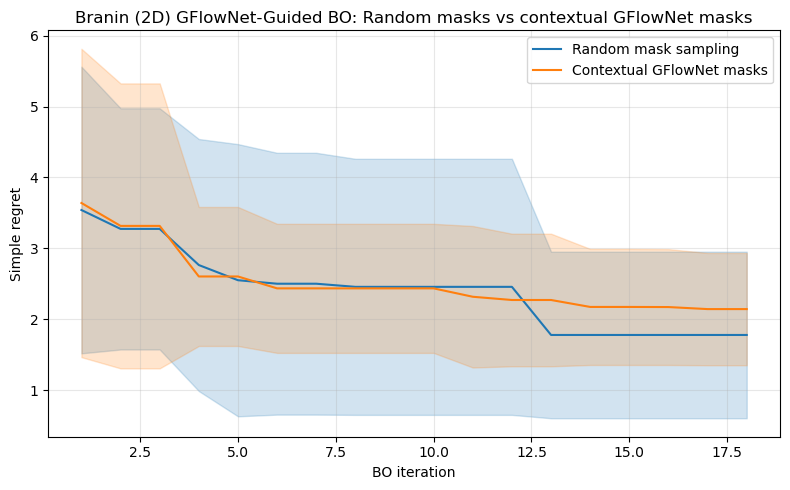
\includegraphics[width=\linewidth,height=0.60\textheight,keepaspectratio]{img/branin_regret_comparison.png}
  \vspace{-0.2em}\par{\TinyCap Random remains stronger.}
  \end{card}
\end{minipage}

\column{0.32\textwidth}
\begin{minipage}[t][0.8\textheight]{\linewidth}\vspace{0pt}
  \begin{card}{Hartmann-6 (6D)}
  \centering
  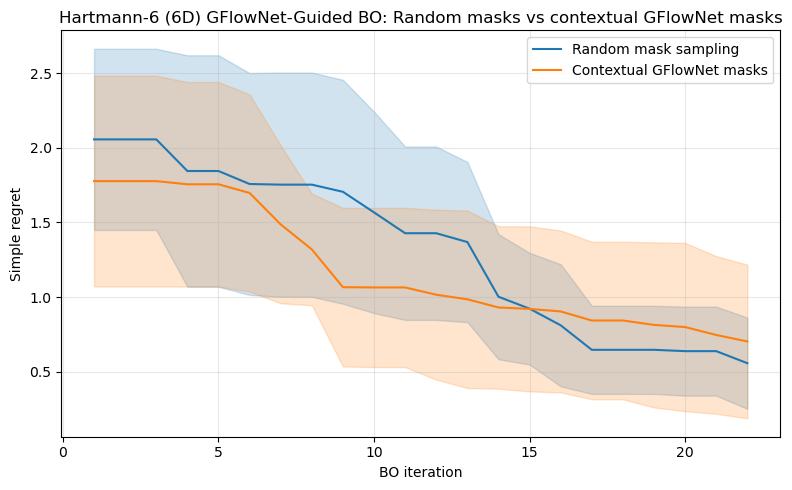
\includegraphics[width=\linewidth,height=0.60\textheight,keepaspectratio]{img/hartmann6_regret_comparison.png}
  \vspace{-0.2em}\par{\TinyCap Random still wins.}
  \end{card}
\end{minipage}

\column{0.32\textwidth}
\begin{minipage}[t][0.8\textheight]{\linewidth}\vspace{0pt}
  \begin{cardG}{Ackley-10 (10D)}
  \centering
  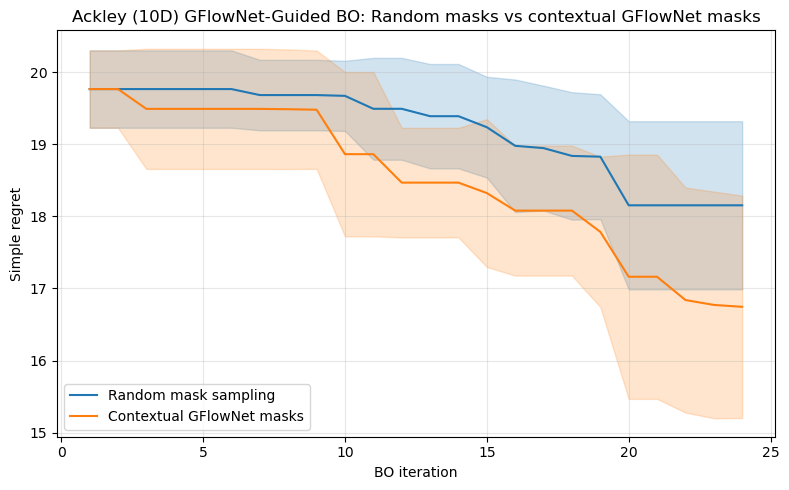
\includegraphics[width=\linewidth,height=0.60\textheight,keepaspectratio]{img/ackley10_regret_comparison.png}
  \vspace{-0.2em}\par{\TinyCap GFlowNet overtakes random and finishes lower.}
  \end{cardG}
\end{minipage}
\end{columns}
\end{frame}

% ------------------------------------------------
\begin{frame}{Final performance summary}
\vspace{-0.55em}
\begin{columns}[T,onlytextwidth]
\column{0.56\textwidth}
\begin{minipage}[t][0.82\textheight]{\linewidth}\vspace{0pt}
  \begin{cardA}{Final regret over 5 seeds}
  \centering
  \begin{tabular}{lccc}
  \toprule
  Benchmark & Random & GFlowNet & Better \\
  \midrule
  Branin (2D) & $1.7813 \pm 1.1734$ & $2.1459 \pm 0.7910$ & Random \\
  Hartmann-6 (6D) & $0.5571 \pm 0.3059$ & $0.7027 \pm 0.5144$ & Random \\
  Ackley (10D) & $18.1526 \pm 1.1661$ & $16.7447 \pm 1.5421$ & GFlowNet \\
  \bottomrule
  \end{tabular}
  \end{cardA}

  \vfill

  \begin{cardG}{Best defensible claim}
  The evidence supports \textbf{benchmark-dependent utility}, not the stronger claim that GFlowNets generally improve neural BO.
  \end{cardG}
\end{minipage}

\column{0.38\textwidth}
\begin{minipage}[t][0.82\textheight]{\linewidth}\vspace{0pt}
  \begin{card}{Readout}
  \begin{itemize}
    \item No universal improvement.
    \item Clear positive evidence only on Ackley-10.
    \item Lower-dimensional benchmarks favor random masks in this setup.
  \end{itemize}
  \end{card}

  \vfill

  \begin{cardW}{Interpretation}
  The controlled protocol did \textbf{not} change the benchmark-level conclusion: mixed outcome persists even after tighter evaluation controls.
  \end{cardW}
\end{minipage}
\end{columns}
\end{frame}

% ------------------------------------------------
\begin{frame}{Ackley-10 diagnostics}
\vspace{-0.55em}
\begin{columns}[T,onlytextwidth]
\column{0.48\textwidth}
\begin{minipage}[t][0.80\textheight]{\linewidth}\vspace{0pt}
  \begin{card}{Best random-mask seed}
  \centering
  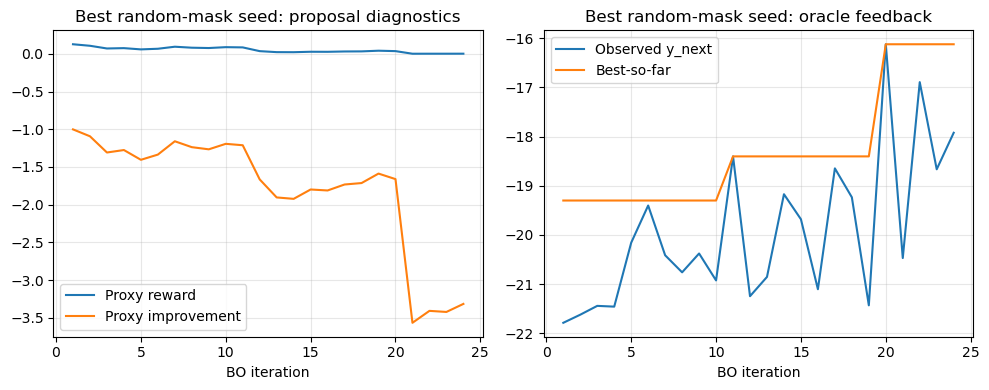
\includegraphics[width=\linewidth,height=0.64\textheight,keepaspectratio]{img/ackley10_random_diagnostics.png}
  \vspace{-0.25em}\par{\TinyCap Proxy scores and best-so-far trajectory for the strongest random run.}
  \end{card}
\end{minipage}

\column{0.48\textwidth}
\begin{minipage}[t][0.80\textheight]{\linewidth}\vspace{0pt}
  \begin{cardG}{Best GFlowNet seed}
  \centering
  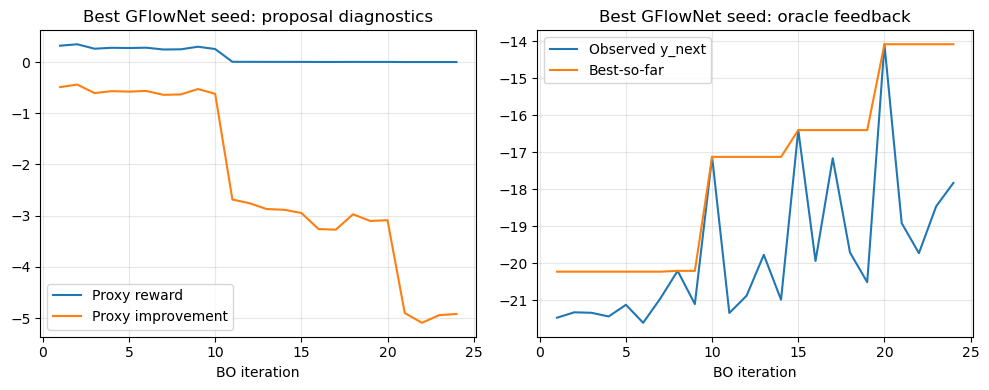
\includegraphics[width=\linewidth,height=0.64\textheight,keepaspectratio]{img/ackley10_gfn_diagnostics.png}
  \vspace{-0.25em}\par{\TinyCap Stronger final best-so-far trajectory, consistent with lower final regret.}
  \end{cardG}
\end{minipage}
\end{columns}
\end{frame}

% ------------------------------------------------
\begin{frame}{Compute trade-off}
\vspace{-0.55em}
\begin{columns}[T,onlytextwidth]
\column{0.56\textwidth}
\begin{minipage}[t][0.82\textheight]{\linewidth}\vspace{0pt}
  \begin{cardW}{Trial-level compute cost}
  \centering
  \begin{tabular}{lcccc}
  \toprule
  Benchmark & Random & GFN & Slowdown & Gain \\
  \midrule
  Branin & 3.75s & 128.07s & $34.11\times$ & $-0.3646$ \\
  Hartmann-6 & 5.77s & 310.73s & $53.85\times$ & $-0.1456$ \\
  Ackley & 7.52s & 509.42s & $67.70\times$ & $+1.4079$ \\
  \bottomrule
  \end{tabular}
  \end{cardW}

  \vfill

  \begin{card}{Per-iteration runtime message}
  Surrogate fitting time is almost identical between methods. Most of the extra cost comes from \textbf{inner-loop GFlowNet training}, not from the base neural BO pipeline.
  \end{card}
\end{minipage}

\column{0.38\textwidth}
\begin{minipage}[t][0.82\textheight]{\linewidth}\vspace{0pt}
  \begin{cardA}{Interpretation}
  \begin{itemize}
    \item On Branin and Hartmann-6, GFlowNet is \textbf{slower and worse}.
    \item Ackley-10 is the only case where the extra cost buys a measurable regret gain.
    \item Even there, the wall-clock overhead is very large.
  \end{itemize}
  \end{cardA}

  \vfill

  \begin{cardG}{Bottom line}
  Query efficiency improves only conditionally, while wall-clock efficiency degrades sharply.
  \end{cardG}
\end{minipage}
\end{columns}
\end{frame}

% ------------------------------------------------
\begin{frame}{Why the mixed result still matters}
\vspace{-0.55em}
\begin{columns}[T,onlytextwidth]
\column{0.47\textwidth}
\begin{minipage}[t][0.82\textheight]{\linewidth}\vspace{0pt}
  \begin{cardA}{Scientifically useful negative result}
  Under a tighter protocol, a mixed result has more weight: it is closer to evidence about the \textbf{method} rather than about a brittle implementation.
  \end{cardA}

  \vfill

  \begin{card}{What the project contributes}
  \begin{itemize}
    \item contextual GFlowNet formulation for sequential dropout-mask generation in BO
    \item more controlled and reproducible benchmark protocol
    \item clearer picture of when learned mask search is worth pursuing
  \end{itemize}
  \end{card}
\end{minipage}

\column{0.47\textwidth}
\begin{minipage}[t][0.82\textheight]{\linewidth}\vspace{0pt}
  \begin{cardW}{Key bottlenecks}
  \begin{itemize}
    \item \textbf{reward alignment}: proxy reward may not track realized BO improvement
    \item \textbf{non-stationarity}: the policy is trained while the BO loop changes
    \item \textbf{compute cost}: 34$\times$--68$\times$ slowdown is substantial
  \end{itemize}
  \end{cardW}

  \vfill

  \begin{card}{Validity limits}
  \begin{itemize}
    \item only 5 seeds
    \item small synthetic benchmark suite
    \item dimensionality is confounded with benchmark identity
  \end{itemize}
  \end{card}
\end{minipage}
\end{columns}
\end{frame}

% ------------------------------------------------
\begin{frame}{Conclusion and future work}
\vspace{-0.55em}
\begin{columns}[T,onlytextwidth]
\column{0.47\textwidth}
\begin{minipage}[t][0.82\textheight]{\linewidth}\vspace{0pt}
  \begin{cardG}{Final claim}
  Under a controlled evaluation protocol, GFlowNet-guided mask sampling:
  \begin{itemize}
    \item helps on Ackley-10
    \item does not beat a matched random-mask baseline on Branin or Hartmann-6
    \item incurs substantial computational overhead in all settings
  \end{itemize}
  \end{cardG}

  \vfill

  \begin{cardA}{Closing line}
  The project's main contribution is a more credible characterization of \textbf{when} learned dropout-mask generation may be useful in neural Bayesian optimization.
  \end{cardA}
\end{minipage}

\column{0.47\textwidth}
\begin{minipage}[t][0.82\textheight]{\linewidth}\vspace{0pt}
  \begin{card}{Future work}
  \begin{itemize}
    \item improve proxy-reward calibration
    \item strengthen contextual conditioning
    \item compare continual fine-tuning vs.\ periodic retraining
    \item add stronger uncertainty-aware baselines
    \item expand the benchmark suite
    \item reduce policy-training cost per BO step
  \end{itemize}
  \end{card}

  \vfill

  \begin{cardW}{Presenter recommendation}
  Keep backup slides only for Branin / Hartmann-6 diagnostics if extra time remains.
  \end{cardW}
\end{minipage}
\end{columns}
\end{frame}

\end{document}
